
\documentclass[aspectratio=1610]{beamer}

\usepackage{def/mypres}


% --- SETUP THEME ---
\mode<presentation>{
    \usetheme{metropolis}
    \setbeamercovered{invisible} %transparent
}

\usecolortheme{seahorse}

\setbeamercolor{title}{fg=black!2!,bg=black}
\setbeamercolor{title separator}{fg=black!2}

%\metroset{background=dark}
\setbeamercolor{normal text}{fg=black!2,bg=rfbg}
\usebeamercolor[fg]{normal text}

%\setsansfont{Latin Modern Roman}
%\setmonofont{Latin Modern Roman}







% --- META ---
\title[Decentralized Target Tracking]{\Large The Dark Side of Decentralized Target Tracking}
\subtitle{\normalsize Unknown Correlations and Communication Constraints} % (optional)
\author{Robin Forsling}
\institute[]{%\inst{1}%
    % Automatic Control, ISY, Linköping University
    % \and
    % AI \& Tactical Autonomy, Advanced Program, Saab Aeronautics
}
\date[]{Speaker's Corner 2024-04-05 %\\
% \begin{tikzpicture}
%     \draw[white](0,0)circle[radius=2];
% \end{tikzpicture}
}
\subject{dtt}



%\pgfdeclareimage[height=1.0cm]{university-logo}{fig/liu_eng/LiU_primary_black.png}
%\logo{\pgfuseimage{university-logo}}



% Delete this, if you do not want the table of contents to pop up at
% the beginning of each subsection:
\AtBeginSubsection[]{
    \begin{frame}<beamer>{Outline}
        \tableofcontents[currentsection,currentsubsection]
    \end{frame}
}




% --- BEGIN DOCUMENT ---
\begin{document}



% TITLE PAGE
\thispagestyle{empty}
\begin{frame}
    \titlepage
\end{frame}

\setbeamercolor{normal text}{fg=rfbg,bg=black!2}
\usebeamercolor[fg]{normal text}


% OUTLINE PAGE
\addtocounter{framenumber}{-1}
% \begin{frame}{Outline}
%     \tableofcontents % You might wish to add the option [pausesections]
% \end{frame}





% --- INTRODUCTION ---
\section{Introduction}

%\subsection[Motivation]{Motivation}


% Summary
\begin{frame}{Introduction}

\begin{columns}

\begin{column}{.5\textwidth}
    \begin{itemize}
        \item Started at Saab 2016
        \item Industrial PhD student at Automatic Control, ISY, LiU between 2018--2023
        \item Main supervisor: Fredrik Gustafsson
        \item Research topic: Target tracking in decentralized sensor networks
        % \item Key words:
        % \begin{itemize}
        %     \item distributed target tracking
        %     \item sensor/data/track fusion
        %     \item network-centric operations
        % \end{itemize}
    \end{itemize}
\end{column}

\begin{column}{.5\textwidth}

    \begin{figure}
        \centering
        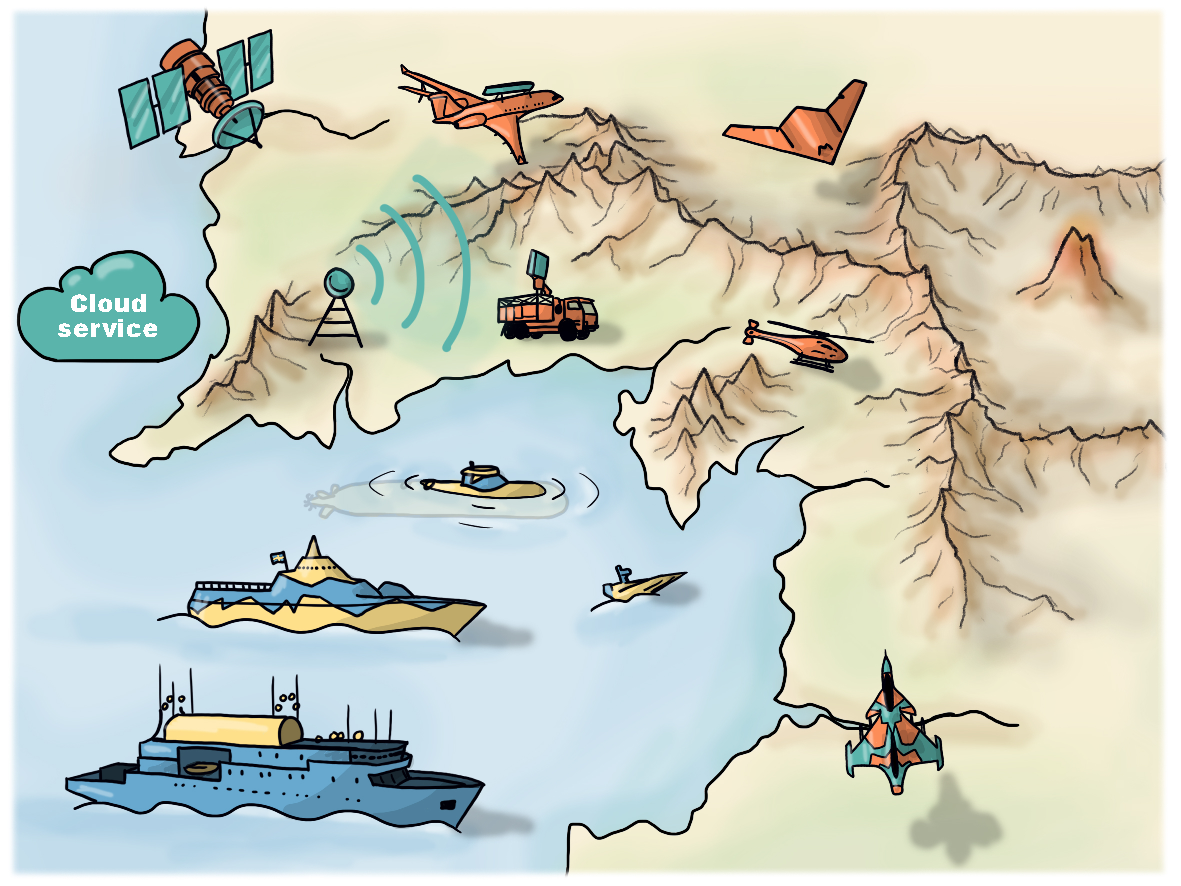
\includegraphics[width=1\textwidth]{figure1-4_network-centric_battle_scene}
    \end{figure}

\end{column}

\end{columns}

\end{frame}


% INTENTIONALLY LEFT BLANK
% \begin{frame}{}
%
% \begin{center}
%     \emph{Intentionally left blank}
% \end{center}
%
% \end{frame}

% TARGET TRACKING
\begin{frame}{A Target Tracking Problem}

\begin{columns}

\begin{column}{.45\textwidth}
    \vspace{-3em}
    \begin{figure}
        \centering
        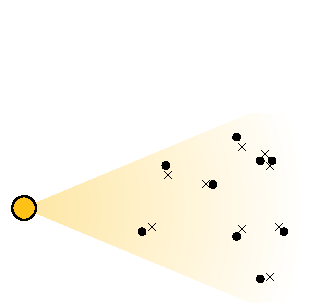
\includegraphics[width=.77\textwidth]{figure1-1a_target_tracking_scene}
        \caption*{Multitarget tracking scene with measurements over multiple time instants}
    \end{figure}
\end{column}

\pause

\begin{column}{.45\textwidth}
    \begin{figure}
        \centering
        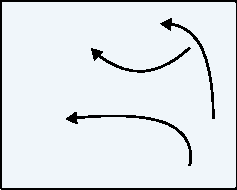
\includegraphics[width=.6\textwidth]{figure1-1b_target_tracking_scene_results}
        \caption*{Refined picture using target tracking algorithms}
    \end{figure}
\end{column}

\end{columns}

\end{frame}


% BASIC TARGET TRACKING SYSTEM
\begin{frame}{Basic Target Tracking System}

\begin{center}
    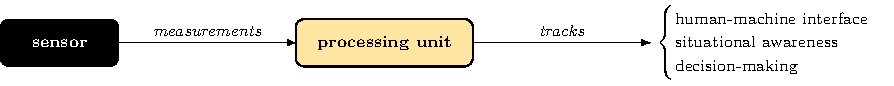
\includegraphics[width=.95\textwidth]{figure1-2_basic_target_tracking_system}
\end{center}

\end{frame}


% THE GREATER PICTURE
\begin{frame}{The Big Picture}

\begin{columns}

\begin{column}{.4\textwidth}
\begin{itemize}
    \item network-centric operations
    \item heterogenous agents: \emph{ships}, \emph{aircraft}, \emph{ground vehicles} etc
    \item asymmetric capabilities
    \item distributed sensors
    \item information exchange
\end{itemize}
\end{column}

\begin{column}{.6\textwidth}
    \begin{figure}
        \centering
        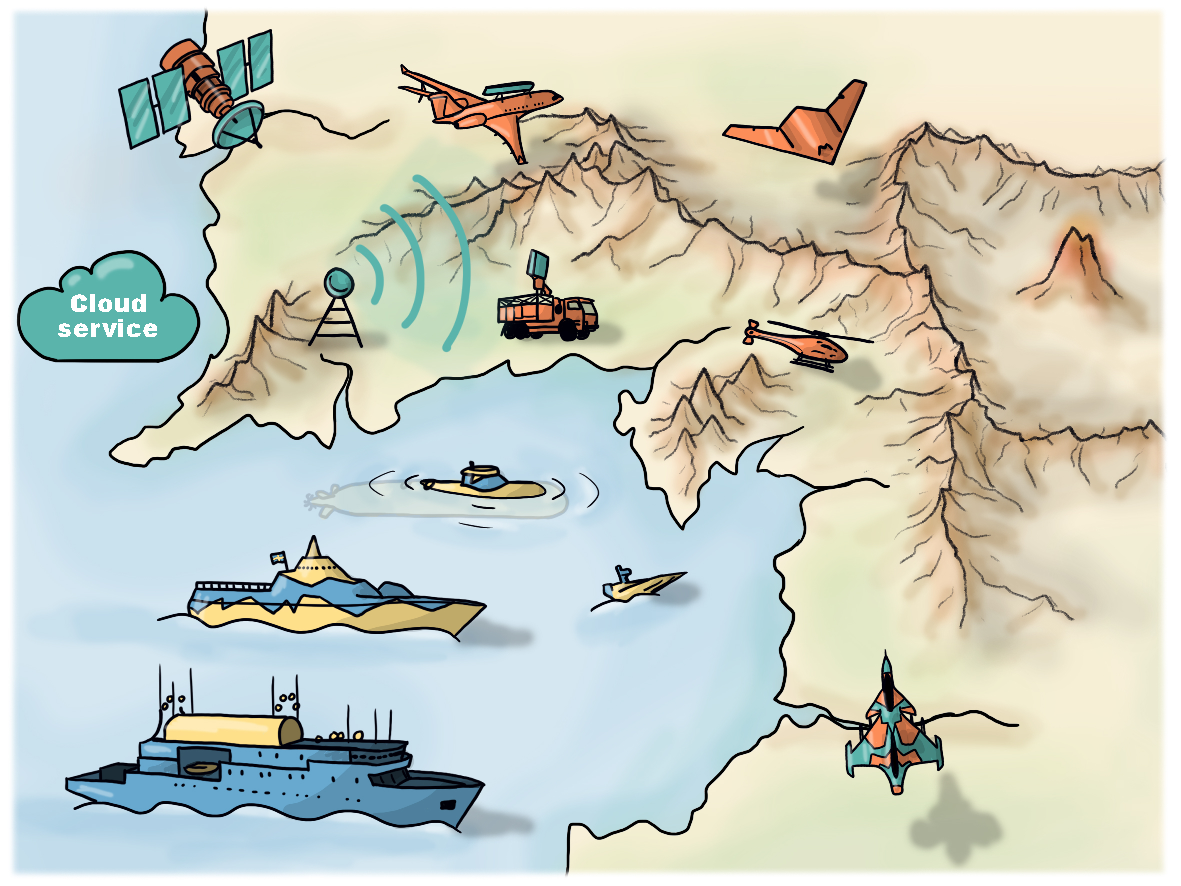
\includegraphics[width=1\textwidth]{figure1-4_network-centric_battle_scene}
    \end{figure}
\end{column}

\end{columns}

\end{frame}


% SENSOR NETWORKS
\begin{frame}{Sensor Network Architectures}

\begin{columns}

\begin{column}{.5\textwidth}
    \begin{center}\textbf{Centralized sensor network}\end{center}
    \begin{figure}
        \centering
        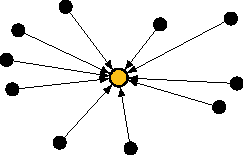
\includegraphics[width=.65\textwidth]{figure1-3a_centralized_sensor_network}
    \end{figure}
    \begin{center}
        \begin{itemize}
            \item possible optimal performance
            \item critical nodes, high complexity
        \end{itemize}
    \end{center}
\end{column}

\begin{column}{.5\textwidth}
    \begin{center}\textbf{Decentralized sensor network}\end{center}
    \begin{figure}
        \centering
        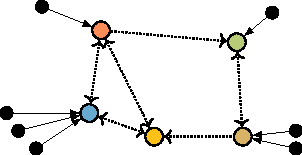
\includegraphics[width=.8\textwidth]{figure1-3b_decentralized_sensor_network}
    \end{figure}
    \begin{center}
        \begin{itemize}
            \item robust, modular, flexible
            \item dependencies (correlations)
        \end{itemize}
    \end{center}
\end{column}

\end{columns}

\end{frame}



% DECENTRALIZED TARGET TRACKING SYSTEM
\begin{frame}{Decentralized Target Tracking: System Perspective}

\begin{center}
    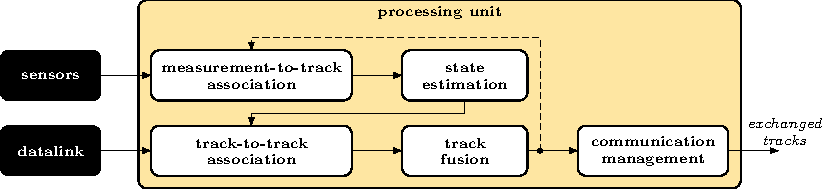
\includegraphics[width=.9\textwidth]{figure1-5_decentralized_target_tracking_system}
\end{center}

\end{frame}


% RESEARCH QUESTIONS
\begin{frame}{Research Problem}

\textbf{Two subproblems}
\begin{enumerate}
    \item robust \alert{track fusion} under unknown correlations
    \item efficient usage of the  \alert{communication resource}
\end{enumerate}

\vspace{1em}

\begin{center}
    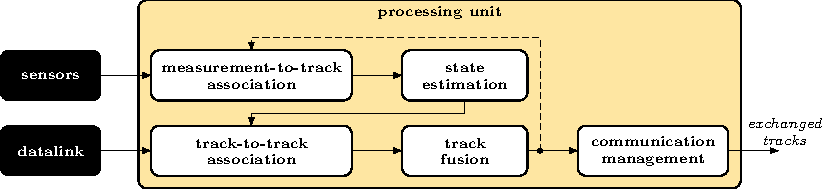
\includegraphics[width=.75\textwidth]{figure1-5_decentralized_target_tracking_system}
\end{center}

\end{frame}


% OUTLINE
\begin{frame}{Outline}

\begin{small}

\textbf{Resources:} \alert{\url{https://github.com/robinforsling/dtt/}}
\begin{itemize}
    \item \matlab source code and thesis summary
\end{itemize}

%\makebox[.5\linewidth]{\rule{\paperwidth}{0.4pt}}

\pause
\vspace{0.5em}

\begin{rfshadedcolorbox}[title={Outline}]{darkgray}

\textbf{Part I:} Track fusion design and evaluation
\begin{itemize}
    \item track fusion methods
    \item evaluation measures and analysis
\end{itemize}

\textbf{Part II:} Communication management design and implementation
\begin{itemize}
    \item two frameworks for reducing the communication load
\end{itemize}

\end{rfshadedcolorbox}
\end{small}

\end{frame}









% --- TACK FUSION DESIGN ---
\section{Part I: Track Fusion Design and Evaluation}

% DSTT
\begin{frame}{Decentralized Single-Target Tracking }

\begin{figure}
    \centering
    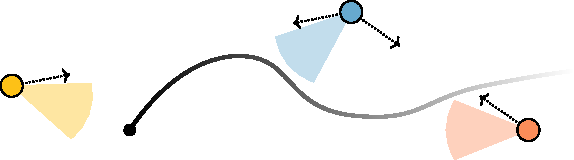
\includegraphics[width=.6\textwidth]{figure3-1_decentralized_single-target_tracking_scenario}
\end{figure}

%\pause

\vspace{1em}

\begin{figure}
    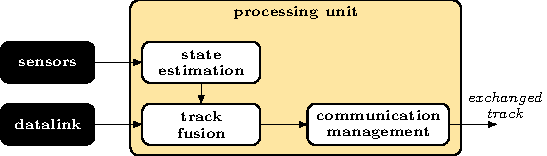
\includegraphics[width=.6\textwidth]{figure3-2_decentralized_single-target_tracking_system}
\end{figure}

\end{frame}


% NOTATION
\begin{frame}{Notation}

\begin{itemize}
    \item $x\in\realsnx$: target state to be estimated
    \item $I$: identity matrix
    \item $A\trnsp$: transpose of matrix (or vector) $A$
    \item $A\inv$: inverse of matrix $A$
    \item $A\succeq0$: $A$ is symmetric positive semidefinite
    \item $A\succ0$: $A$ is symmetric positive definite
    \item $\EV(\bfa)$: expected value of $\bfa$
    \item $\cov(\bfa)$: covariance (matrix) of $\bfa$
\end{itemize}

\end{frame}


% ESTIMATE MODEL
\begin{frame}{Estimate Model}

By $(y_i,R_i)$ we denote the local estimate/track in \ith agent, model as
\begin{align*}
    y_i &= H_i x + v_i &
    R_i &= \cov(\bfv_i)
\end{align*}
where $R_i$ is the covariance of the noise $v_i$

\vspace{1em}

In this presentation $H_i=I$ is assumed for simplicity, \ie, $y_i\in\realsnx$

%\pause
\vspace{1em}

\alert{linear model, but not necessarily Cartesian!}

\end{frame}


% TF: OPTIMAL
\begin{frame}{Track Fusion: Optimal Method}

Consider:
\begin{itemize}
    \item $(y_1,R_1)$ and $(y_2,R_2)$ are to be fused
    \item $R_{12}=R_{21}\trnsp=\cov(\bfy_1,\bfy_2)$ is the cross-covariance between the estimates
\end{itemize}

An optimal fusion method is given by:
\begin{align*}
    \xhat &= K_1y_1 + K_2y_2 &
    P &= R_1 - K_2SK_2\trnsp
\end{align*}
where $K_1=I-K_2$, $K_2=(R_1-R_{12})S\inv$, and $S=R_1+R_2-R_{12}-R_{12}\trnsp$

\end{frame}


% TF: DSN
\begin{frame}{Track Fusion: Decentralized Sensor Networks}

Why not use the optimal fusion method? \alert{$R_{12}$ is unknown!}

\vspace{2em}

\begin{figure}
    \centering
    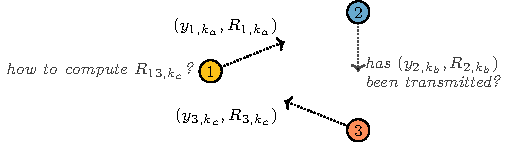
\includegraphics[width=1.25\textheight]{figure3-5_tracking_correlations}
\end{figure}

\end{frame}


% TF: NAIVE SOLUTION
\begin{frame}{Track Fusion: Naive Solution}

The naive solution: \alert{assume that $R_{12}=0$}

\vspace{1em}

Optimal fusion given that $R_{12}=0$:
\begin{align*}
    \xhat &= P\left(R_1\inv y_1 + R_2\inv y_2  \right) &
    P &= \left(R_1\inv + R_2\inv \right)\inv
\end{align*}

%\pause

\vspace{1em}

If $R_{12}\neq0$, the \alert{uncertainty $P$ is underestimated} --- double counting of information

\end{frame}




% TF: UNKNOWN XCORR
\begin{frame}{Track Fusion: Conservative Estimators}

\textbf{Issues}:
\begin{itemize}
    \item unknown correlations
    \item if nonzero correlations are neglected the uncertainty $P$ is underestimated
\end{itemize}

\textbf{Possible solution:} \emph{conservative estimators}

\begin{rfshadedcolorbox}[title={Conservative Estimate}]{myyellow!200!}
    An estimate $(\xhat,P)$ of $x$ is \emph{conservative} if
    \begin{equation*}
        P - \EV(\tbfx\tbfx\trnsp) \succeq 0
    \end{equation*}
    where $\tbfx=\hbfx-x$ is the error
\end{rfshadedcolorbox}

\end{frame}


% CONSERVATIVE AND NON-CONSERVATIVE
\begin{frame}{Conservative and Non-Conservative Estimates}

\begin{figure}
    \begin{tikzpicture}[scale=.5]
        
\def\drawtrue{\draw[ultra thick,dashed,black]}
\def\drawcons{\draw[ultra thick,mydarkgreen]}
\def\drawnon{\draw[ultra thick,myred]}

\def\Ptrue{(0,0)ellipse[x radius = 4, y radius = 1.5, rotate = 20];}

\def\xleg{-5}
\def\yleg{4.5}
\def\lleg{1}
\def\sleg{12}





% --- FIGURE ---
\BFS


% LEFT
\drawtrue\Ptrue
\drawcons (0,0) ellipse [x radius = 5, y radius = 2, rotate = 25];
\node at (0,0) {$P\succeq\EV(\tbfx\tbfx\trnsp)$};


% RIGHT
\begin{scope}[xshift=16cm]
	
\drawtrue\Ptrue
\drawnon (0,0) ellipse [x radius = 5, y radius = 2, rotate = -25];	
\node at (0,0) {$P^n\not\succeq\EV(\tbfx\tbfx\trnsp)$};
	
\end{scope}


% LEGEND
\drawcons({\xleg},\yleg)--({\xleg+\lleg},\yleg) node [right,black] {$P$};
\drawtrue ({\xleg+\sleg},\yleg)--({\xleg+\lleg+\sleg},\yleg) node [right,black] {$\EV(\tbfx\tbfx\trnsp)$};
\drawnon ({\xleg+2*\sleg},\yleg)--({\xleg+\lleg+2*\sleg},\yleg) node [right,black] {$P^n$};




\EFS

    \end{tikzpicture}
\end{figure}

\end{frame}


% TF: CF
\begin{frame}{Track Fusion: Conservative Methods}

\textbf{Task:} Fuse $(y_1,R_1)$ and $(y_2,R_2)$, where $R_{12}$ is unknown

\vspace{2em}

\begin{columns}

\begin{column}{0.475\textwidth}

\textbf{Conservative fusion methods:}
\begin{itemize}
    \item \textcolor{clrci}{\textbf{covarance intersection}}
    \item \textcolor{clrle}{\textbf{largest ellipsoid method}}
    \item \textcolor{gray}{inverse covariance intersection}
    \item \textcolor{gray}{split covariance intersection}
    \item $\cdots$
\end{itemize}

\end{column}

\begin{column}{0.475\textwidth}
\begin{figure}
    \begin{tikzpicture}[scale=0.75]
        
% R1 and R2
\draw[thick,black](0,0)ellipse[x radius=3,y radius=1,rotate=30];
\draw[thick,black](0,0)ellipse[x radius=3,y radius=1,rotate=120];

% CI
\draw[ultra thick,clrci](0,0)circle[radius=1.3416];

% LE
\draw[ultra thick,clrle](0,0)circle[radius=1.0];

    \end{tikzpicture}
\end{figure}
\end{column}

\end{columns}

\end{frame}


% COVARIANCE INTERSECTION
\begin{frame}{Covariance Intersection}

\begin{rfshadedcolorbox}[title={Covariance Intersection}]{clrci}
The estimates are fused using \emph{covariance intersection} (\abbrCI) according to
\begin{align*}
    \xhat &= P\left( \omega R_1\inv y_1 + (1-\omega)R_2\inv y_2 \right) &
    P &= \left(\omega R_1\inv + (1-\omega)R_2\inv \right)\inv
\end{align*}
where $\omega\in[0,1]$ is computed by solving
\begin{equation*}
    \begin{aligned}
        & \underset{\omega}{\minimize} & & J(P)
    \end{aligned}
\end{equation*}
\end{rfshadedcolorbox}

\pause

\vspace{1em}

Similar in structure to the naive fusion method:
\begin{align*}
    \xhat &= P\left(R_1\inv y_1 + R_2\inv y_2  \right) &
    P &= \left(R_1\inv + R_2\inv \right)\inv
\end{align*}

\end{frame}


% LARGEST ELLIPSOID Method
\begin{frame}{Largest Ellipsoid Method}

\begin{rfshadedcolorbox}[title={Largest Ellipsoid Method},fontupper=\footnotesize]{clrle}
    The estimates are fused using the \emph{largest ellipsoid} (\abbrLE) method according to
    \begin{enumerate}
        \item Factorize $R_1=U_1\Sigma_1U_1\trnsp$ and let $T_1=\Sigma_1\invsqrt U_1\trnsp$. Factorize $T_1R_2T_1\trnsp=U_2\Sigma_2U_2\trnsp$ and let $T_2=U_2\trnsp$.
        \item Transform using $T=T_2T_1$ according to
            \begin{align*}
                 z_1 &= Ty_1 & C_1 &= TR_1T\trnsp=I &
                 z_2 &= Ty_2 & C_2 &= TR_2T\trnsp
            \end{align*}
        \item For each $i=1,\dots,\nx$, compute
            \begin{equation*}
                \left([z]_i,[C]_{ii}\right) =
                    \begin{cases}
                        \left([z_1]_i,1\right), & \text{ if } 1 \leq [C_2]_{ii},\\
                        \left([z_2]_i,[C_2]_{ii}\right), & \text{ if } 1 > [C_2]_{ii}.
                    \end{cases}
            \end{equation*}
        \item Transform back:
            \begin{align*}
                \xhat &= T\inv z &
                P &= T\inv C T\invtrnsp
            \end{align*}
    \end{enumerate}
\end{rfshadedcolorbox}

\end{frame}


% MC EVALUATION
\begin{frame}{Monte Carlo Evaluation}

\emph{Monte Carlo} (\abbrMC) based approach for evaluation:
\begin{enumerate}
	\item Specify local sensors, local state estimation filters, and communication pattern.
	\item Specify the considered track fusion methods.
	\item Define a metrics for tracking performance and conservativeness.
	\item Define characteristic target trajectories.
	\item Tune the local filters for the characteristic trajectories.
	\item Using \abbrMC simulations, evaluate each fusion method with respect to performance and conservativeness.
\end{enumerate}

An estimate at the \ith \abbrMC run at time $k$ is denoted $(\xhat_k^i,P_k^i)$

\end{frame}


% PERFORMANCE EVALUATION
\begin{frame}{Performance Evaluation}

\emph{Root mean squared error} (\abbrRMSE) is a common measure for performance
\begin{itemize}
    \item requires the true state to be known --- \alert{cannot be computed online}
\end{itemize}

\pause

\vspace{1em}

\begin{rfshadedcolorbox}[title={Root Mean Trace}]{darkgray}
    The sampled \emph{root mean trace} (\abbrRMT) at time $k$ is defined as
    \begin{equation*}
        \rmt_k = \sqrt{\frac{1}{M}\sum_{i=1}^M \trace(P_k^i) }
    \end{equation*}
\end{rfshadedcolorbox}



\end{frame}


% CONSERVATIVENESS EVALUATION
\begin{frame}{Conservativeness Evaluation}

Since $P=LL\trnsp\succ0$, the Cholesky factor $L$ is invertible such that
\begin{equation*}
    P \succeq \EV(\tbfx\tbfx\trnsp) \iff I \succeq L\inv \EV(\tbfx\tbfx\trnsp) L\invtrnsp
\end{equation*}

\vspace{1em}

Hence $(\xhat,P)$ is conservative iff
\[
    \lambdamax\left(L\inv\EV(\tbfx\tbfx\trnsp) L\invtrnsp\right) \leq 1
\]
$\lambdamax(A)$ denotes the largest eigenvalue of a matrix $A$

\end{frame}

\begin{frame}{Conservativeness Evaluation}

\begin{rfshadedcolorbox}[title={Conservativeness Index}]{darkgray}
    The sampled \emph{conservativeness index} (\abbrCOIN) at time $k$ is defined as
    \begin{equation*}
        \coin_k = \lambdamax\left( \underbrace{\frac{1}{M} \sum_{i=1}^M (L_k^i)\inv\xtilde_k^i(\xtilde_k^i)\trnsp(L_k^i)\invtrnsp }_{\calC_k} \right)
    \end{equation*}
    where $L_k^i(L_k^i)\trnsp=P_k^i$, $\xtilde_k^i$ is the error in the \ith \abbrMC run, and $\calC_k$ is the sampled normalized estimation error squared matrix
\end{rfshadedcolorbox}

\pause

\vspace{1em}

\alert{Want $\coin_k$ to be smaller than or equal to 1}

\end{frame}



% EVALUATION
\begin{frame}{Evaluation Scenario}

\begin{figure}
    \begin{tikzpicture}[scale=.5]
        

\def\ragent{0.5}

\def\xa{-2,1}
\def\xb{5,0}
\def\xt{3,8}

\def\xsu{2,1.0}
\def\xsl{2,-1.0}


% --- FIGURE ---
\BFS


% TARGET:
\drawtargettrajectory[smooth](3,8)--(3.206,7.886)--(3.416,7.781)--(3.631,7.684)--(3.849,7.595)--(4.070,7.515)--(4.294,7.444)--(4.521,7.381)--(4.750,7.328)--(4.981,7.283)--(5.214,7.248)--(5.447,7.222)--(5.682,7.205)--(5.917,7.197)--(6.153,7.198)--(6.388,7.209)--(6.622,7.228)--(6.855,7.257);
\node at (\xt) {\mycircle{black}};


% MEAS COV:
\drawdefaultellipse{clra}(\xt)ellipse[x radius = 2.447, y radius = .367, rotate = 54.5];
\drawdefaultellipse{clrb}(\xt)ellipse[x radius = 2.447, y radius = .352, rotate = 104.0];


% AGENT 1:
\draw\sensoropt{clra} [rotate around={54:(\xa)}] (\xa) -- ($(\xa)+(\xsu)$) to [out=-60,in=60] ($(\xa)+(\xsl)$) -- cycle;
\drawcomarrow[->] (\xa)--($(\xa)!.25!(\xb)$);	
\drawagent{clra} (\xa) circle [radius = \ragent];


% AGENT 2:
\draw\sensoropt{clrb} [rotate around={104:(\xb)}] (\xb) -- ($(\xb)+(\xsu)$) to [out=-60,in=60] ($(\xb)+(\xsl)$) -- cycle;
\drawcomarrow[->] (\xb)--($(\xb)!.25!(\xa)$);	
\drawagent{clrb} (\xb) circle [radius = \ragent];


\EFS

%($(#2)+({#5*cos(#3)},{#5*sin(#3)})$) arc (#3:#4:#5); }	  
%\def\middlepoint(#1)(#2){($(#1)!.5!(#2)$)}   
    \end{tikzpicture}
\end{figure}

\end{frame}


% RESULTS
\begin{frame}{Evaluation Results}

\begin{figure}
    \begin{tikzpicture}[xscale=.25,yscale=1.2]
        
\newcommand*\drawci{\draw[very thick,clrci]}
\newcommand*\drawle{\draw[very thick,clrle]}
\newcommand*\drawlkf{\draw[very thick,clrlkf]}
\newcommand*\drawnkf{\draw[very thick,clrnaive,dotted]}

\def\plotcommand{plot[smooth]coordinates}
\def\plotcommandb{plot[]coordinates}

\def\ks{1}
\def\kend{19}
\def\ymin{0}

\def\xleg{2}
\def\yleg{4.5}
\def\lleg{1.5}
\def\sleg{12}

\def\xs{25cm}
\def\ysa{-1.875cm}
\def\ysb{-4cm}

\def\addxlabel(#1){\node at (#1) {$k$};}
\def\addxticks{\foreach \x in {4,8,...,16} {\drawxtick(\x,\ymin);\node [below] at (\x,\ymin) {\x};}}
\def\addyticks{\foreach \y in {0.5,1.0,1.5,2.0,2.5,3.0,3.5} {\drawytick(\ks,\y);\node [left] at (\ks,\y) {\y};}}
\def\drawframe{\drawcoordinateframe(\ks,\ymax)--(\ks,\ymin)--(\kend,\ymin);}

\def\s{3.5};





% --- FIGURE ---
\BFS


\addxlabel(10,-0.5)
\addxlabel(35,-0.5)

\def\ymin{0}; \def\ymax{4}


% RMT:
\draw[very thick,gray](\ks,1)--(\kend,1);
\drawci\plotcommand{(2,1.677)(4,1.373)(6,1.437)(8,1.422)(10,1.371)(12,1.326)(14,1.310)(16,1.317)(18,1.331)};
\drawle\plotcommand{(2,1.234)(4,1.032)(6,1.055)(8,1.038)(10,1.009)(12,0.989)(14,0.983)(16,0.988)(18,0.995)};
\drawnkf\plotcommand{(2,1.166)(4,0.765)(6,0.696)(8,0.596)(10,0.485)(12,0.393)(14,0.335)(16,0.303)(18,0.284)};
\drawlkf\plotcommand{(2,3.434)(4,2.876)(6,3.103)(8,3.276)(10,3.209)(12,3.007)(14,2.807)(16,2.660)(18,2.559)};

\addxticks
\addyticks
\drawframe
\node[rotate=90] at (-2.5,2) {RMT};


% COIN:
\begin{scope}[xshift=25cm]

\draw[very thick,gray](\ks,1)--(\kend,1);
\drawci\plotcommand{(2,0.520)(4,0.645)(6,0.572)(8,0.578)(10,0.633)(12,0.672)(14,0.692)(16,0.678)(18,0.650)};
\drawle\plotcommand{(2,1.068)(4,0.990)(6,0.963)(8,1.018)(10,1.085)(12,1.097)(14,1.072)(16,1.038)(18,0.996)};
\drawnkf\plotcommand{(2,1.131)(4,3.781)};
\drawlkf\plotcommand{(2,1.131)(4,1.091)(6,1.022)(8,0.986)(10,0.993)(12,1.029)(14,1.043)(16,1.017)(18,0.978)};

\addxticks
\addyticks
\drawframe
\node[rotate=90] at (-2.5,2) {COIN};

\end{scope}







% LEGEND:
\drawci({\xleg},\yleg)--({\xleg+\lleg},\yleg) node [right,black] {\abbrCI};
\drawle ({\xleg+\sleg},\yleg)--({\xleg+\lleg+\sleg},\yleg) node [right,black] {\abbrLE};
\drawnkf ({\xleg+2*\sleg},\yleg)--({\xleg+\lleg+2*\sleg},\yleg) node [right,black] {naive fusion};
\drawlkf ({\xleg+3*\sleg},\yleg)--({\xleg+\lleg+3*\sleg},\yleg) node [right,black] {local filter};




\EFS

    \end{tikzpicture}
\end{figure}

\end{frame}






% --- COMMUNICATION MANAGEMENT ---
\section{Part II: Communication Management Design and Implementation}


% CM: INTRO
\begin{frame}{Communication Management: Data Reduction}

\begin{figure}
    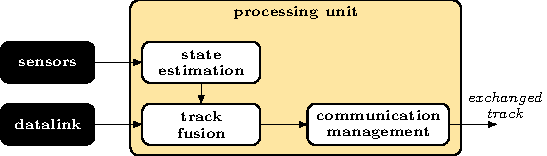
\includegraphics[width=.6\textwidth]{figure3-2_decentralized_single-target_tracking_system}
\end{figure}

\textbf{Two main approaches:}
\begin{itemize}
    \item diagonal covariance approximation (\abbrDCA)
    \item dimension-reduction (\abbrDR)
\end{itemize}

\end{frame}


% DCA
\begin{frame}{Diagonal Covariance Approximation}

\textbf{Problem:}
\begin{itemize}
    \item Agent~2 is about to transmit $(y_2,R_2)$ to Agent~1
    \item limited communication capacity: the data $(y_2,R_2)$ must be reduced
\end{itemize}

%\pause
\vspace{1em}

\textbf{Observation:} $y_i$ scales as $\nx$ and $R_i$ as $\nx^2$

%\pause
\vspace{1em}

\textbf{Simple solution:} exchange $(y_2,D_2)$ where $D_2$ is diagonal --- essentially an $\nx$-dimensional vector

\end{frame}


% DCA
\begin{frame}{Diagonal Covariance Approximation: Example}

Let $R_2=\BBSM4&1\\1&1\EBSM$ and $D_2=\BBSM4&0\\0&1\EBSM$

\begin{figure}
    \centering
    \begin{tikzpicture}
        
\def\Riopt{[ultra thick,clrkf]}
\def\Diopt{[ultra thick,dashed,clrkf]}
\def\Dsiopt{[ultra thick,mydarkgreen]}

\def\xleg{4}
\def\yleg{0.45}
\def\sleg{0.45}
\def\lleg{0.4}




% --- FIGURE ---
\BFS


\draw[white,opacity=0] (-6,-1) rectangle (6,1);

\draw\Riopt (0,0) ellipse [x radius = 2.07, y radius = 0.83, rotate = -163.15];
\draw\Diopt (0,0) ellipse [x radius = 2, y radius = 1];
\draw\Dsiopt (0,0) ellipse [x radius = 2.82, y radius = 1.41];

\draw\Riopt ({\xleg},{\yleg})--({\xleg+\lleg},{\yleg}) node [right,black] {$R_2$};
\draw\Diopt ({\xleg},{\yleg-\sleg})--({\xleg+\lleg},{\yleg-\sleg}) node [right,black] {$D_2$};
\draw\Dsiopt ({\xleg},{\yleg-2*\sleg})--({\xleg+\lleg},{\yleg-2*\sleg}) node [right,black] {$\Ds_2=2D_2$};

\node at (0,0) {$D_2\not\succeq R_2$};
\node [left] at (-2.82,0) {$\Ds_2\succeq R_2$};


\EFS

    \end{tikzpicture}
\end{figure}

\pause
\vspace{1em}

Agent~2 preserves conservativeness if $(y_2,\Ds_2)$ is exchanged

\end{frame}


% DCA: 2 OPTIONS
\begin{frame}{Diagonal Covariance Approximation: Two Options}

Two options are considered:
\begin{itemize}
	\item Agent~2 transmits $(y_2,\Ds_2)$ to Agent~1, where $\Ds_2\succeq R_2$. In this case, Agent~2 has already preserved conservativeness, and hence, Agent~1 can use the received estimate directly without any additional action.
	\item Agent~2 transmits $(y_2,D_2)$ to Agent~1. In this case, Agent~1 must explicitly handle that $D_2\not\succeq R_2$ to ensure conservativeness after track fusion.
\end{itemize}

\end{frame}


% D1: DCA-EIG
\begin{frame}{Diagonal Covariance Approximation: Eigenvalue Based Scaling}

\begin{rfshadedcolorbox}[title={Eigenvalue Based Scaling}]{myyellow!200!}
    \begin{equation*}
    \begin{aligned}
    	& \underset{s}{\minimize} & & s \\
    	& \subjectto & & \Ds_2 = sD_2 \succeq R_2.
    \end{aligned}
    \end{equation*}
\end{rfshadedcolorbox}

%\pause
\vspace{1em}

The solution is
\[
    s^\star=\lambdamax(D_2\invsqrt R_2D_2\invsqrt)
\]

\end{frame}


% D2: DCA-HYP
\begin{frame}{Diagonal Covariance Approximation: Hyperrectangle Enclosing}

Agent~1 receives $(y_2,D_2)$ from Agent~2
\begin{itemize}
    \item Assume $R_2=\BBSM4&1\\1&1\EBSM$ such that $D_2=\BBSM4&0\\0&1\EBSM$
\end{itemize}

\begin{figure}
    \centering
    \begin{tikzpicture}[scale=.85]
        
\newcommand*\drawBellipse{\draw[gray,thick]}
\newcommand*\drawhyperrectangle{\draw[thick,black]}
\newcommand{\drawdiagonalbound}[1]{\draw[ultra thick,#1]}

\def\xl{2}
\def\yl{1}

\def\xleg{5.25}
\def\yleg{0.75}
\def\sleg{0.5}
\def\lleg{0.5}



% --- FIGURE ---
\BFS

\def\bbx{8}; \def\bby{1}
%\draw [white,opacity=0] (-\bbx,-\bby) rectangle (\bbx,\bby);

\foreach \r/\ly/\lx in {154.90/0.40/2.20,156.58/0.55/2.17,158.49/0.67/2.13,160.67/0.76/2.10,163.15/0.83/2.07,165.96/0.89/2.05,169.10/0.94/2.03,172.53/0.97/2.01,176.20/0.99/2.00,0.00/1.00/2.00,-176.20/0.99/2.00,-172.53/0.97/2.01,-169.10/0.94/2.03,-165.96/0.89/2.05,-163.15/0.83/2.07,-160.67/0.76/2.10,-158.49/0.67/2.13,-156.58/0.55/2.17,-154.90/0.40/2.20} {
	\drawBellipse[opacity=0.2] (0,0) ellipse [x radius = \lx, y radius = \ly, rotate = \r];}

\foreach \r/\ly/\lx in {154.90/0.40/2.20,164.52/0.87/2.06,0.00/1.00/2.00,-164.52/0.87/2.06,-154.90/0.40/2.20} {
	\drawBellipse[opacity=0.5] (0,0) ellipse [x radius = \lx, y radius = \ly, rotate = \r];}

% Box
\drawhyperrectangle (-\xl,-\yl) rectangle (\xl,\yl);

% Bounds
\drawdiagonalbound{clra}(0,0)ellipse[x radius = 4.47, y radius = 1.12];
\drawdiagonalbound{clrb}(0,0)ellipse[x radius = 3.65, y radius = 1.20];
\drawdiagonalbound{clrc}(0,0)ellipse[x radius = 3.16, y radius = 1.29];
\drawdiagonalbound{clrd}(0,0)ellipse[x radius = 2.83, y radius = 1.41];

% Legend
\begin{scriptsize}
\drawdiagonalbound{clra} ({\xleg},{\yleg})--({\xleg+\lleg},{\yleg}) node [right,black] {$\Domega_2|_{\omega_1=0.2,\omega_2=0.8}$};
\drawdiagonalbound{clrb} ({\xleg},{\yleg-\sleg})--({\xleg+\lleg},{\yleg-\sleg}) node [right,black] {$\Domega_2|_{\omega_1=0.3,\omega_2=0.7}$};
\drawdiagonalbound{clrc} ({\xleg},{\yleg-2*\sleg})--({\xleg+\lleg},{\yleg-2*\sleg}) node [right,black] {$\Domega_2|_{\omega_1=0.4,\omega_2=0.6}$};
\drawdiagonalbound{clrd} ({\xleg},{\yleg-3*\sleg})--({\xleg+\lleg},{\yleg-3*\sleg}) node [right,black] {$\Domega_2|_{\omega_1=\omega_2=0.5}$};
% \drawBellipse ({\xleg},{\yleg-4*\sleg})--({\xleg+\lleg},{\yleg-4*\sleg}) node [right,black] {$B\in\calA$};
% \drawhyperrectangle ({\xleg},{\yleg-5*\sleg})--({\xleg+\lleg},{\yleg-5*\sleg}) node [right,black] {$\calR$};
\end{scriptsize}

%\node at (0,0) {$\calA$};

\EFS

    \end{tikzpicture}
\end{figure}

%\pause
%\vspace{1em}

The parametrization given by
\begin{equation*}
    D_2^\omega = \BBM \frac{4}{\omega_1}&0 \\ 0&\frac{1}{\omega_2} \EBM
\end{equation*}
where $\omega_i>0$ and $\sum_i\omega_i=1$

\end{frame}


% DR: BASIC IDEA
\begin{frame}{Dimension Reduction: Basic Idea}

Instead of transmitting $(y_2,R_2)$ Agent~2 can transmit $(\yM,\RM)$ where
\begin{align*}
    \yM &= \M y_2 &
    \RM &= \M R_2\Mt
\end{align*}
and $\M\in\realsmnx$ is a ''wide matrix'', \ie, $m<\nx$

\vspace{1em}

This is a \emph{dimension reduction} problem

\end{frame}


% DR: CHOOSING PSI
\begin{frame}{Dimension Reduction: Designing $\M$}

How to choose $\M$? \alert{Optimize for fusion performance!}

\vspace{1em}

Assume that $(y_1,R_1)$ and $(\yM,\RM)$ are fused according to
\begin{align*}
    \xhat &= P\left( R_1\inv y_1 + \Mt\RM\inv\yM \right) &
    P &= \left(R_1\inv + \Mt\RM\inv\M \right)\inv
\end{align*}
which is optimal given that the estimates are uncorrelated

\end{frame}


% DR: SOLUTION
\begin{frame}{Dimension Reduction: Designing $\M$}

\begin{rfshadedcolorbox}[title={Fusion Optimal Dimension Reduction}]{myorange}
    A fusion optimal $\Mopt$ is computed by solving
    \begin{equation*}
    	\begin{aligned}
    		& \underset{\M}{\minimize} & & \trace(P).
    	\end{aligned}
    \end{equation*}
    where $P=\left(R_1\inv + \Mt\RM\inv\M \right)\inv$
\end{rfshadedcolorbox}

\vspace{1em}

The solution is given by an eigenvalue problem!

\end{frame}


% DR VS DCA
\begin{frame}{Communication Reduction}

Let $\ndca$, $\ndr$, and $\nfull$ denote the number of parameters to be transmitted using \abbrDCA, \abbrDR, and full estimates, respectively

\begin{figure}
    \centering
    %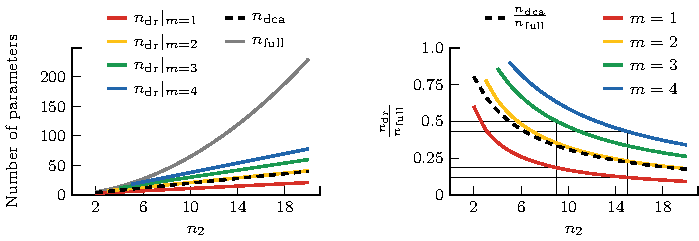
\includegraphics[width=.95\textwidth]{figure5-1_dr_communication_reduction}
    \begin{tikzpicture}
        
\newcommand*\drawnfull{\draw[very thick,gray]}
\newcommand*\drawndca{\draw[very thick,dashed,black]}
\newcommand{\drawndr}[1]{\draw[very thick,#1]}
\newcommand{\drawratio}[1]{\draw[very thick,#1]}

\def\xlega{3}
\def\xlegb{13}
\def\yleg{300}
\def\lleg{1.6}
\def\sleg{40}

\def\addxlabel(#1){\node at (#1) {$\nx$};}




% --- FIGURE ---
\BFS


% LEFT
\begin{scope}[xscale=0.2,yscale=0.01]

\foreach \y in {0,50,...,200} {\drawytick(0,\y);\node [left] at (0,\y) {\y};}
\foreach \x in {2,6,...,18} {\drawxtick(\x,0);\node [below] at (\x,0) {\x};}
\drawcoordinateframe(0,250)--(0,0)--(21,0);
\addxlabel(10.5,-60)
\node [rotate=90] at (-5,125) {Number of parameters};

\drawnfull plot [smooth] coordinates {(2,5)(3,9)(4,14)(5,20)(6,27)(7,35)(8,44)(9,54)(10,65)(11,77)(12,90)(13,104)(14,119)(15,135)(16,152)(17,170)(18,189)(19,209)(20,230)};
\drawndr{clrm1} plot [smooth] coordinates {(2,3)(3,4)(4,5)(5,6)(6,7)(7,8)(8,9)(9,10)(10,11)(11,12)(12,13)(13,14)(14,15)(15,16)(16,17)(17,18)(18,19)(19,20)(20,21)};
\drawndr{clrm2} plot [smooth] coordinates {(3,7)(4,9)(5,11)(6,13)(7,15)(8,17)(9,19)(10,21)(11,23)(12,25)(13,27)(14,29)(15,31)(16,33)(17,35)(18,37)(19,39)(20,41)};
\drawndr{clrm3} plot [smooth] coordinates {(4,12)(5,15)(6,18)(7,21)(8,24)(9,27)(10,30)(11,33)(12,36)(13,39)(14,42)(15,45)(16,48)(17,51)(18,54)(19,57)(20,60)};
\drawndr{clrm4} plot [smooth] coordinates {(5,18)(6,22)(7,26)(8,30)(9,34)(10,38)(11,42)(12,46)(13,50)(14,54)(15,58)(16,62)(17,66)(18,70)(19,74)(20,78)};
\drawndca plot [smooth] coordinates {(2,4)(3,6)(4,8)(5,10)(6,12)(7,14)(8,16)(9,18)(10,20)(11,22)(12,24)(13,26)(14,28)(15,30)(16,32)(17,34)(18,36)(19,38)(20,40)};

\drawndr{clrm1} ({\xlega},{\yleg})--({\xlega+\lleg},{\yleg}) node [right,black] {$\ndr|_{m=1}$};
\drawndr{clrm2} ({\xlega},{\yleg-\sleg})--({\xlega+\lleg},{\yleg-\sleg}) node [right,black] {$\ndr|_{m=2}$};
\drawndr{clrm3} ({\xlega},{\yleg-2*\sleg})--({\xlega+\lleg},{\yleg-2*\sleg}) node [right,black] {$\ndr|_{m=3}$};
\drawndr{clrm4} ({\xlega},{\yleg-3*\sleg})--({\xlega+\lleg},{\yleg-3*\sleg}) node [right,black] {$\ndr|_{m=4}$};

\drawndca ({\xlegb},{\yleg})--({\xlegb+\lleg},{\yleg}) node [right,black] {$\ndca$};
\drawnfull ({\xlegb},{\yleg-\sleg})--({\xlegb+\lleg},{\yleg-\sleg}) node [right,black] {$\nfull$};

\end{scope}


% RIGHT
\begin{scope}[xscale=0.2,yscale=2.5,xshift=32cm]

\def\yleg{1.2}
\def\sleg{0.16}

\drawsupportline(0,0.5)--(9,0.5)--(9,0);
\drawsupportline(0,0.185)--(9,0.185);
\drawsupportline(0,0.430)--(15,0.430)--(15,0);
\drawsupportline(0,0.119)--(15,0.119);

\foreach \y in {0,0.25,0.5,0.75,1.0} {\drawytick(0,\y);\node [left] at (0,\y) {\y};}
\foreach \x in {2,6,...,18} {\drawxtick(\x,0);\node [below] at (\x,0) {\x};}
\drawcoordinateframe(0,1)--(0,0)--(21,0);
\addxlabel(10.5,-.24)
\node [rotate=90] at (-5,0.5) {$\frac{\ndr}{\nfull}$};

\drawratio{clrm1} plot [smooth] coordinates {(2,0.600)(3,0.444)(4,0.357)(5,0.300)(6,0.259)(7,0.229)(8,0.205)(9,0.185)(10,0.169)(11,0.156)(12,0.144)(13,0.135)(14,0.126)(15,0.119)(16,0.112)(17,0.106)(18,0.101)(19,0.096)(20,0.091)};
\drawratio{clrm2} plot [smooth] coordinates {(3,0.778)(4,0.643)(5,0.550)(6,0.481)(7,0.429)(8,0.386)(9,0.352)(10,0.323)(11,0.299)(12,0.278)(13,0.260)(14,0.244)(15,0.230)(16,0.217)(17,0.206)(18,0.196)(19,0.187)(20,0.178)};
\drawratio{clrm3} plot [smooth] coordinates {(4,0.857)(5,0.750)(6,0.667)(7,0.600)(8,0.545)(9,0.500)(10,0.462)(11,0.429)(12,0.400)(13,0.375)(14,0.353)(15,0.333)(16,0.316)(17,0.300)(18,0.286)(19,0.273)(20,0.261)};
\drawratio{clrm4} plot [smooth] coordinates {(5,0.900)(6,0.815)(7,0.743)(8,0.682)(9,0.630)(10,0.585)(11,0.545)(12,0.511)(13,0.481)(14,0.454)(15,0.430)(16,0.408)(17,0.388)(18,0.370)(19,0.354)(20,0.339)};
\drawndca plot [smooth] coordinates {(2,0.800)(3,0.667)(4,0.571)(5,0.500)(6,0.444)(7,0.400)(8,0.364)(9,0.333)(10,0.308)(11,0.286)(12,0.267)(13,0.250)(14,0.235)(15,0.222)(16,0.211)(17,0.200)(18,0.190)(19,0.182)(20,0.174)};

\drawndr{clrm1} ({\xlegb},{\yleg})--({\xlegb+\lleg},{\yleg}) node [right,black] {$m=1$};
\drawndr{clrm2} ({\xlegb},{\yleg-\sleg})--({\xlegb+\lleg},{\yleg-\sleg}) node [right,black] {$m=2$};
\drawndr{clrm3} ({\xlegb},{\yleg-2*\sleg})--({\xlegb+\lleg},{\yleg-2*\sleg}) node [right,black] {$m=3$};
\drawndr{clrm4} ({\xlegb},{\yleg-3*\sleg})--({\xlegb+\lleg},{\yleg-3*\sleg}) node [right,black] {$m=4$};

\drawndca ({\xlega},{\yleg})--({\xlega+\lleg},{\yleg}) node [right,black] {$\frac{\ndca}{\nfull}$};

\end{scope}


\EFS

    \end{tikzpicture}
\end{figure}


\end{frame}


% --- SUMMARY ---
\section*{Summary}


\begin{frame}{Summary}

\begin{small}

\textbf{Excluded material:}
\begin{itemize}
    \item the \abbrCLUE framework
    \item common information estimate --- keeping track of network common information
    \item practical and theoretical aspects related to the data reduction techniques
%    \item $\cdots$
\end{itemize}

\vskip0pt plus.5fill

\textbf{Related resources:} \alert{\url{https://github.com/robinforsling/dtt/}}
\begin{itemize}
%    \item it is quite short, read it!
    \item \matlab library source code for all examples and simulation
    \item thesis summary
    \item posters, papers, bibliography, figures
\end{itemize}

\end{small}

\end{frame}


\end{document}
